\documentclass[
	% -- opções da classe memoir --
	12pt,				% tamanho da fonte
	openright,			% capítulos começam em pág ímpar (insere página vazia caso preciso)
	oneside,			% para impressão em apenas anverso. Oposto a twoside
	%twoside,			% para impressão em verso e anverso. Oposto a oneside
	a4paper,			% tamanho do papel. 
	% -- opções da classe abntex2 --
	%chapter=TITLE,		% títulos de capítulos convertidos em letras maiúsculas
	%section=TITLE,		% títulos de seções convertidos em letras maiúsculas
	%subsection=TITLE,	% títulos de subseções convertidos em letras maiúsculas
	%subsubsection=TITLE,% títulos de subsubseções convertidos em letras maiúsculas
	% -- opções do pacote babel --
	english,			% idioma adicional para hifenização
	francais,			% idioma adicional para hifenização
	spanish,			% idioma adicional para hifenização
	brazil				% o último idioma é o principal do documento
	]{abntex2}

% Evita linhas orfãs e viúvas
\widowpenalty=10000
\clubpenalty=10000

\usepackage{lmodern}			% Usa a fonte Latin Modern
\usepackage[T1]{fontenc}		% Selecao de codigos de fonte.
\usepackage[utf8]{inputenc}		% Codificacao do documento (conversão automática dos acentos)
\usepackage{lastpage}			% Usado pela Ficha catalográfica
\usepackage{indentfirst}		% Indenta o primeiro parágrafo de cada seção.
\usepackage{color}				% Controle das cores
\usepackage{graphicx}			% Inclusão de gráficos
\usepackage{microtype} 			% para melhorias de justificação
\usepackage{lipsum}				% para geração de dummy text
\usepackage[brazilian,hyperpageref]{backref}	% Paginas com as citações na bibl
\usepackage[alf]{abntex2cite}					% Citações padrão ABNT
\usepackage{graphicx}
\usepackage{tikz}
\usetikzlibrary{shapes,arrows,chains}
\usepackage[]{mcode}
\usepackage{multirow}
\usepackage{array}
\usepackage{todonotes}
\usepackage{longtable}
\usepackage{rotating}
\usepackage{caption}
\usepackage{pbox}
\usepackage{pdfpages}
\usepackage{float}
\usepackage{tikz}
\usepackage{circuitikz}	
\usetikzlibrary{babel}	% Necessário para o funcionamento do circuitikz

\usepackage[brazil]{babel}		% idiomas
\addto\captionsbrazil{
	%% ajusta nomes padroes do babel
	\renewcommand{\bibname}{Refer\^encias Bibliogr\'aficas}
	\renewcommand{\indexname}{\'Indice Remissivo}
	\renewcommand{\listfigurename}{Lista de Figuras}
	\renewcommand{\listtablename}{Lista de Tabelas}
	\renewcommand{\listadesiglasname}{Lista de Abreviaturas e Siglas}
	%% ajusta nomes usados com a macro \autoref
	\renewcommand{\pageautorefname}{p\'agina}
	\renewcommand{\sectionautorefname}{se{\c c}\~ao}
	\renewcommand{\subsectionautorefname}{subse{\c c}\~ao}
	\renewcommand{\paragraphautorefname}{par\'agrafo}
	\renewcommand{\subsubsectionautorefname}{subse{\c c}\~ao}
}

% ---
% Configurações do pacote backref
% Usado sem a opção hyperpageref de backref
\renewcommand{\backrefpagesname}{Citado na(s) página(s):~}
% Texto padrão antes do número das páginas
\renewcommand{\backref}{}
% Define os textos da citação
\renewcommand*{\backrefalt}[4]{
	\ifcase #1 %
		Nenhuma citação no texto.%
	\or
		Citado na página #2.%
	\else
		Citado #1 vezes nas páginas #2.%
	\fi}%
% ---

\definecolor{blue}{RGB}{0,114,189}
\definecolor{orange}{RGB}{217,83,25}
\definecolor{yellow}{RGB}{237,177,32}
\definecolor{purple}{RGB}{126,47,142}
\definecolor{green}{RGB}{119,172,48}
\definecolor{lightBlue}{RGB}{77,190,238}
\definecolor{red}{RGB}{162,20,47}
\definecolor{black}{RGB}{0,0,0}

% informações do PDF
\makeatletter
\hypersetup{
     	%pagebackref=true,
		pdftitle={\@title}, 
		pdfauthor={\@author},
    	pdfsubject={\imprimirpreambulo},
	    pdfcreator={LaTeX with abnTeX2},
		pdfkeywords={abnt}{latex}{abntex}{abntex2}{trabalho acadêmico}, 
		colorlinks=true,	% false: boxed links; true: colored links
    	linkcolor=black,	% color of internal links
    	citecolor=black,	% color of links to bibliography
    	filecolor=black,	% color of file links
		urlcolor=black,
		bookmarksdepth=4
}
\makeatother

% --- 
% Espaçamentos entre linhas e parágrafos 
% --- 
% O tamanho do parágrafo é dado por:
\setlength{\parindent}{1.3cm}
% Controle do espaçamento entre um parágrafo e outro:
\setlength{\parskip}{0.2cm}  % tente também \onelineskip


\titulo{Modelagem de Sistemas Não Lineares de Áudio Através de Espaço de Estados e Filtros Digitais Wave}
\autor
{
	UNIVERSIDADE FEDERAL DO RIO GRANDE DO SUL\\
	ESCOLA DE ENGENHARIA\\
	DEPARTAMENTO DE ENGENHARIA ELÉTRICA\\
	\vspace*{4\baselineskip} 
	MATHEUS OLIVEIRA DA SILVA
}
\local{Porto Alegre}
\data{2017}
\orientador{Prof. Dr. Adalberto Schuck Jr.}
\coorientador{}
\instituicao{}
\preambulo{Projeto de Diplomação apresentado ao Departamento de Engenharia Elétrica da Escola de Engenharia da Universidade Federal do Rio Grande do Sul, como requisito parcial para Graduação em Engenharia Elétrica}

\makeindex
\begin{document}
\selectlanguage{brazil}
\frenchspacing 

\imprimircapa
\imprimirfolhaderosto*

%\begin{fichacatalografica}
%	\includepdf{fichaCatalog.pdf}
%\end{fichacatalografica}

%=========================================================================
% FOLHA DE APROVAÇÃO
%=========================================================================

\begin{folhadeaprovacao}
	\begin{center}
		{\ABNTEXchapterfont\large{MATHEUS OLIVEIRA DA SILVA}}
		
		\vspace*{\fill}
		\begin{center}
			\ABNTEXchapterfont\bfseries\Large\imprimirtitulo
		\end{center}
		
		\vspace*{\fill}
		\hspace{.45\textwidth}
		\begin{minipage}{.5\textwidth}
			\imprimirpreambulo
		\end{minipage}%
	\end{center}
	
	\assinatura{\textbf{\imprimirorientador} \\ Orientador - UFRGS} 
	\todo{Atualizar Chefe do Departamento}
	\assinatura{\textbf{Prof. Dr. Ály Ferreira Flores Filho} \\ Chefe do Departamento de Engenharia Elétrica (DELET) - UFRGS}
	
	\todo{Atualizar data da apresentação}
	\begin{center}
		Aprovado em 15 de Janeiro de 2018.
	\end{center}
	
	BANCA EXAMINADORA	
	\assinatura{\textbf{Banca 1} \\ UFRGS}
	\assinatura{\textbf{Banca 2} \\ UFRGS}
	\assinatura{\textbf{Banca 3} \\ UFRGS}
\end{folhadeaprovacao}

%=========================================================================
% DEDICATÓRIA
%=========================================================================

\begin{dedicatoria}
	\vspace*{\fill}
	\centering
	\noindent
	\textit{Aos que me apoiaram durante minha graduação, \\e também aos que duvidaram de minha capacidade, \\me dando forças para prová-los errados} \vspace*{\fill}
\end{dedicatoria}

%=========================================================================
% AGRADECIMENTOS
%=========================================================================

\begin{agradecimentos}
tbd
\end{agradecimentos}

%=========================================================================
% EPÍGRAFE
%=========================================================================

\begin{epigrafe}
	\vspace*{\fill}
	\begin{flushright} 
		\textit{We live in a society exquisitely dependent on science and technology,\\ in which hardly anyone knows anything about science and technology.}\\ \vspace{\onelineskip}
		Carl Sagan, The Demon-Haunted World
	\end{flushright}
\end{epigrafe}

%=========================================================================
% RESUMOS
%=========================================================================

% resumo em português
\setlength{\absparsep}{18pt} % ajusta o espaçamento dos parágrafos do resumo
\begin{resumo}
	Distorções em sistemas de áudio causadas por não linearidades são responsáveis pela sonoridade característica de alguns estilos musicais, por isso é importante seu estudo e compreensão. Estes "defeitos" são originalmente causados por sistemas valvulados analógicos, porém estes são de difícil mobilidade e grandes consumidores de energia. Con o poder computacional disponível atualmente é possível a reprodução destes sistemas analógicos digitalmente de forma ininteligível para o ouvido humano. Assim é atraente a ideia de simular estes com o objetivo de obter sistemas mais portáteis e econômicos.

	\vspace{\onelineskip}
	\textbf{Palavras-chave}: Sistemas não lineares. Filtros Digitais Wave. Espaço de Estados.
\end{resumo}

% resumo em inglês
\begin{resumo}[Abstract]
 \begin{otherlanguage*}{english}
	
   \vspace{\onelineskip}
   \noindent 
   \textbf{Keywords}:
 \end{otherlanguage*}
\end{resumo}

%=========================================================================
% SUMÁRIOS
%=========================================================================

% inserir lista de ilustrações
\pdfbookmark[0]{\listfigurename}{lof}
\listoffigures*
\cleardoublepage

% inserir lista de tabelas
\pdfbookmark[0]{\listtablename}{lot}
\listoftables*
\cleardoublepage

% inserir lista de abreviaturas e siglas
\begin{siglas}
	\item[LIT]		\emph{Linear Invariante no Tempo}
	\item[SNL]		\emph{Sistema Não Linear}
	\item[FDO]		\emph{Filtro Digital de Onda}

\end{siglas}

% inserir o sumario
\pdfbookmark[0]{\contentsname}{toc}
\tableofcontents*
\cleardoublepage

\textual
%=========================================================================
% INTRODUÇÃO
	\chapter{Introdução}
%=========================================================================

Sistemas lineares invariantes no tempo (LIT) já foram amplamente estudados por autores conhecidos como \citeonline{Haykin2003} e  \citeonline{Oppenheim1997}, tanto são que esses autores já fazem parte da bibliografia básica de disciplinas de graduação. O grande atrativo para o estudo de sistemas LIT é a simplicidade com que se pode obter a saída esperada para uma entrada tendo a resposta impulsiva do sistema, já que as únicas alterações causadas por sistemas LTI são na fase e amplitude do sinal de entrada.

Sistemas não lineares (SNL) por outro lado, apresentam saídas mais complexas pois adicionam à saída do sinal componentes com frequências múltiplas às do sinal de entrada, que são conhecidas como harmônicas. De acordo com \citeonline{Zolzer2002} efeitos não lineares são usados por músicos em diversos dispositivos como microfones amplificadores e sintetizadores.

O princípio do uso de SNLs para áudio foi com a construção de amplificadores baseados em válvulas termiônicas a partir da década de 1950 como indicado por \citeonline{Ferreira2016}. O problema destes componentes é seu peso e consumo de energia, assim foi natural sua substituição por componentes semicondutores mais leves, baratos e confiáveis, porém até hoje as distorções geradas por válvulas são vistas como superiores às geradas por semicondutores por audiófilos, um estudo sobre estas diferenças foi feito por \citeonline{Hamm1973}. Para tentar emular o som gerado por estas válvulas termiônicas em sistemas semicondutores passou a ser comum a construção de pedais de efeitos que são ligados em série com o sistemas de áudio, tendo esses a vantagem de serem mais baratos e de mais fácil transporte. O próximo passo nessa evolução é o uso de sistemas digitais para a modelagem dessas não linearidades com o objetivo de facilitar ainda mais o uso dessa tecnologia, essa enfim será a proposta deste trabalho.

Para o modelamento de SNLs são comuns 3 diferentes abordagens: modelamento de caixa branca, onde se tem total conhecimento do circuito sendo modelado; caixa cinza, onde se usa algum conhecimento do circuito para a modelagem; e caixa preta, onde não é utilizado nenhuma característica do circuito para a modelagem. \citeonline{Eichas2015} propões um modelo de caixa preta onde um ruído branco é injetado no SNL a ser modelado e a saída deste é comparada com a de um sistema paramétrico que é adaptado de maneira a minimizar o erro quadrático entre ambas. 

%=========================================================================
% FUNDAMENTAÇÃO TEÓRICA
	\chapter{Fundamentação Teórica}
%=========================================================================

	%=========================================================================
	\section{Filtros Digitais de Onda}
	%=========================================================================
	
	%=========================================================================
	\subsection{Condições de realização}
	%=========================================================================
	\label{secCondicoesDeRealizacao}
	
	%=========================================================================
	\subsection{Transformação bilinear}
	%=========================================================================
	
	\begin{equation}
		\label{eqTransformacaoBilinear}
		s = \frac{1}{2.f_s}.\frac{z-1}{z+1}
	\end{equation}
	
	%=========================================================================
	\subsection{Variáveis de onda}
	%=========================================================================
	
	Usando as equações de Kirchhoff componentes são descritos de acordo com sua resistência (ou impedância), a tensão entre seus terminais e a corrente que atravessa o mesmo, e a relação entre essas grandezas é dada pela lei de Ohm conforme indicado na Equação \ref{eqLeiDeOhm} e a descrição de um componente qualquer mostrada na Figura \todo{Adicionar figura demonstrando como funciona um componente no domínio K}.
	
	\begin{equation}
	\label{eqLeiDeOhm}
		V = R . I
	\end{equation} 
	
	Deste ponto em diante neste trabalho, essas grandezas serão definidas como parte do domínio K (de acordo com as leis de Kirchhoff). 
	
	\cite{Fettweis1986}	Dentro da teoria de FDO é definido um novo domínio denominado W (do inglês Wave) onde componentes e suas conexões são definidos de acordo com ondas incidentes e refletidas de suas portas e pela resistência dessas portas. As variáveis de corrente e tensão do domínio K são mapeadas como onda de tensão incidente \textit{A} e onda refletida \textit{B} no domínio W conforme indicado pelas transformações lineares nas Equações \ref{eqOndaADefinicao} e \ref{eqOndaBDefinicao}, e a descrição de um componente qualquer no domínio W é indicada na Figura \todo{Adicionar figura mostrando componente no domínio W}.
	
	\begin{equation}
	\label{eqOndaADefinicao}
		A = V + I . R_p
	\end{equation}
	\begin{equation}
	\label{eqOndaBDefinicao}
		B = V - I . R_p
	\end{equation}
	
	Sendo $R_p$ a resistência da porta como será descrito na próxima seção.
	
	Levando em consideração as variáveis de onda definidas nas Equações \ref{eqOndaADefinicao} e \ref{eqOndaBDefinicao}, é possível obter novamente os valores de tensão e corrente do domínio K a partir dos valores do domínio W de acordo com as Equações \ref{eqTensaoDefinicao} e \ref{eqCorrenteDefinicao}.
	
	\begin{equation}
		\label{eqTensaoDefinicao}
		V = \frac{A + B}{2}
	\end{equation} 
	\begin{equation}
		\label{eqCorrenteDefinicao}
		I = \frac{A - B }{2 . R_p}
	\end{equation}
	
	Também é possível definir as variáveis onda levando em consideração ondas de corrente ou potência, porém este trabalho não fará essas definições já que de maneira geral a bibliografia encontrada costuma considerar apenas ondas de tensão. Caso o leitor deseje uma referência às definições de outros tipos de onda no domínio W é indicado o trabalho de \citeonline{Kubin1985}. 
	
	%=========================================================================
	\subsection{Componentes de uma porta no domínio W}
	%=========================================================================
	Neste capítulo será definida a descrição no domínio W para resistores, capacitores, fontes de tensão com resistência em série e fontes de corrente com resistência em série, pois estes são os componentes relevantes para este trabalho. Essas formulações, e outras para componentes passivos de duas portas, são definidos em \citeonline{Yeh2008} e um guia bastante didático para a obtenção destes valores é dado em \citeonline{Bogason2017}.
	 
	 	%=========================================================================
		\subsubsection{Resistores}
		%=========================================================================
	
	Resistores são definidos no domínio K conforme indicado pela Equação \ref{eqDefinicaoResistor}
	
	\begin{equation}
		\label{eqDefinicaoResistor}
		Z_r = \frac{V}{I}
	\end{equation}
	
	Utilizando-se das relações entre tensão, corrente e as variáveis de onda do domínio W definidas nas Equações \ref{eqTensaoDefinicao} e \ref{eqCorrenteDefinicao}, pode-se obter os valores para \textit{A} e \textit{B} conforme indicado nas Equações \ref{edDefinicaoResistorW1} e \ref{eqDefinicaoResistorW2}.
	
	\begin{equation}
		\label{edDefinicaoResistorW1}
		Z_r = \frac{\frac{A+B}{2}}{\frac{A-B}{2.R_p}}
	\end{equation}  
	
	\begin{equation}
		\label{eqDefinicaoResistorW2}
		B = \frac{Z_r-R_p}{Z_r+R_p}.A
	\end{equation}
	
	A Equação \ref{eqDefinicaoResistorW2} pode ser escrita no domínio do tempo conforme a Equação \ref{eqDefinicaoResistorTempo}
	
	\begin{equation}
		\label{eqDefinicaoResistorTempo}
		b[n] = \frac{Z_r-R_p}{Z_r+R_p}.a[n]
	\end{equation}
	
	De acordo com a Equação \ref{eqDefinicaoResistorTempo} a onda refletida de um resistor no domínio W $B$ é relacionada instantaneamente à onda incidente $A$ por um fator $\frac{Z_r-R_p}{Z_r+R_p}$, é desejável que essa relação direta não exista de maneira a facilitar que a condição 1 de realização de filtros digitais, conforme indicado na Seção \ref{secCondicoesDeRealizacao}, seja satisfeita, para isso se define a resistência de entrada $R_p$ no domínio W como sendo igual a resistência $Z_r$ do domínio K. Desta maneira um resistor é completamente definido no domínio W pelas Equações \ref{eqBResistorDominioW} e \ref{eqRResistorDominioW} e a Figura \ref{figResistorDominioW} mostra o funcionamento interno deste componente e seu símbolo.
	
	\begin{equation}
		\label{eqBResistorDominioW}
		B = 0
	\end{equation}   
	\begin{equation}
		\label{eqRResistorDominioW}
		R_p = Z_r
	\end{equation}
	
	\begin{figure}[h]
		\label{figResistorDominioW}
		\caption{Funcionamento interno e símbolo de um resistor no domínio W}
		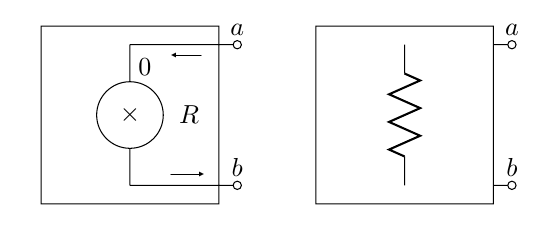
\includegraphics[scale=0.5]{images/resistor}
		\centering
		\caption*{Fonte: Modificado de \cite{Bogason2017}}
	\end{figure}
	
	É importante ressaltar que, mesmo não tendo nenhuma onda refletida, os resistores ainda afetam o comportamento dos circuitos ao alterar o coeficiente de reflexão de conexões série e paralelo com a resistência de sua porta de entrada conforme será mostrado na Seção \ref{secConexoesNoDominioW}.
	
		%=========================================================================
		\subsubsection{Capacitores}
		%=========================================================================
	
	Capacitores são definidos no domínio K em frequência conforme indicado na Equação
	
	\begin{equation}
		\label{eqCapacitorDefinicaoDominioK}
		Z_c = \frac{1}{s.C} = \frac{V}{I}
	\end{equation}
	
	Novamente utilizando-se das relações indicadas nas Equações \ref{eqTensaoDefinicao} e \ref{eqCorrenteDefinicao} obtêm-se as relações para o domínio W conforme indicado nas Equações \ref{eqDefinicaoCapacitorW1} e \ref{eqDefinicaoCapacitorW2}.
	
	\begin{equation}
		\label{eqDefinicaoCapacitorW1}
		\frac{1}{s.C} = \frac{\frac{A+B}{2}}{\frac{A-B}{2.R_p}}
	\end{equation}
	
	\begin{equation}
		\label{eqDefinicaoCapacitorW2}
		B = \frac{1-s.C.R_p}{1+s.C.R_p}.A
	\end{equation}
	
	Utilizando a transformação bilinear dada na Equação \ref{eqTransformacaoBilinear} para digitalizar a Equação \ref{eqDefinicaoCapacitorW2} tem-se as Equações \ref{eqDefinicaoCapacitorW3} e \ref{eqDefinicaoCapacitorW4}
	
	
	\begin{equation}
		\label{eqDefinicaoCapacitorW3}
		B = \frac{1-\frac{1}{2.f_s}.\frac{z-1}{z+1}.C.R_p}{1+\frac{1}{2.f_s}.\frac{z-1}{z+1}.C.R_p}.A
	\end{equation} 
	
	\begin{equation}
		\label{eqDefinicaoCapacitorW4}
		B = \frac{(1-2.f_s.C.R_p)+(1+2.f_s.C.R_p).z^{-1}}{(1+2.f_s.C.R_p)+(1-2.f_s.C.R_p).z^{-1}}.A
	\end{equation}
	
	E finalmente, essa relação entre as ondas \textit{A} e \textit{B} pode ser descrita no domínio tempo conforme a Equação \ref{eqDefinicaoCapacitorTempo}
	
	\begin{equation}
		\label{eqDefinicaoCapacitorTempo}
		b[n] = \frac{((1-2.f_s.C.R_p).a[n]+(1+2.f_s.C.R_p).a[n-1]-(1-2.f_s.C.R_p).b[n-1])}{1+2.f_s.C.R_p}	\end{equation}
	
	Percebe-se pela Equação \ref{eqDefinicaoCapacitorTempo} que a onda refletida em um capacitor é relacionada instantaneamente à onda incidente por um fator $\frac{1-2.f_s.C.R_p}{1+2.f_s.C.R_p}$. Afim de anular essa reflexão instantânea se define a resistência $R_p$ como sendo $\frac{1}{2.f_s.C}$. Assim um capacitor pode ser definido no domínio W conforme indicado nas Equações \ref{eqBCapacitorDominioW} e \ref{eqRCapacitorDominioW} e na Figura \ref{figCapacitorDominioW} e mostrado o funcionamento interno e o símbolo utilizado para capacitores no domínio W.
	
	\begin{equation}
	\label{eqBCapacitorDominioW}
		B = z^{-1}.A
	\end{equation}
	\begin{equation}
	\label{eqRCapacitorDominioW}
		R_p = \frac{1}{2.f_s.C}
	\end{equation}
	
	\begin{figure}[h]
		\label{figCapacitorDominioW}
		\caption{Funcionamento interno e símbolo de um capacitor no domínio W}
		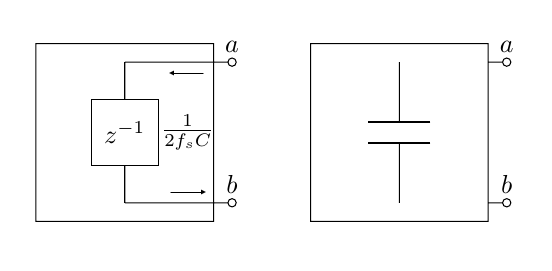
\includegraphics[scale=0.5]{images/capacitor}
		\centering
		\caption*{Fonte: Modificado de \cite{Bogason2017}}
	\end{figure}
	
		%=========================================================================
		\subsubsection{Fonte de tensão com resistência não nula}
		%=========================================================================
	\cite{Yeh2008} Fontes de tensão isolada tem, invariavelmente, uma relação instantânea entre onda incidente e onda refletida, para evitar esse efeito indesejado, é comum na literatura agrupar fontes de tensão com resistores em série conforme o circuito da Figura \ref{figFonteTensaoModelada}. Esse circuito pode ser modelado no domínio K conforme o indicado na Equação \ref{eqFonteTensaoDominioK}.
	
	\begin{equation}
		\label{eqFonteTensaoDominioK}
		V = V_s + R_s.I
	\end{equation}
	
	 \begin{figure}[h]
		\label{figFonteTensaoModelada}
		\caption{Fonte de tensão com resistor em série a ser modelada}
		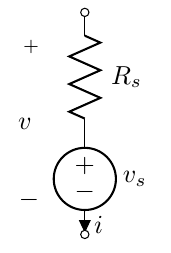
\includegraphics[scale=0.5]{images/fonteTensaoModelada}
		\centering
		\caption*{Fonte: Modificado de \cite{Bogason2017}}
	\end{figure}
	
	Utilizando-se das transformações lineares indicadas nas Equações \ref{eqTensaoDefinicao} e \ref{eqCorrenteDefinicao} e resolvendo as equações de maneira similar à feita anteriormente para resistores e capacitores tem-se que a onde refletida para esse circuito é dada pela Equação 
	
	\begin{equation}
		\label{eqFonteTensaoDominioW}
		B = 2.\frac{R_p.V_s}{R_p+R_s}-A.\frac{R_p-R_s}{R_p+R_s}
	\end{equation}
	
	Pode-se então definir $R_p = R_s$ de maneira a simplificar a equação e evitar a relação instantânea entre onde incidente e onda refletida. Então, uma fonte de tensão em série com um resistor pode ser descrita no domínio W conforme as Equações \ref{eqBFonteTensao} e \ref{eqRFonteTensao} e a Figura \ref{figFonteTensaoDominioW} mostra seu funcionamento e o símbolo utilizado para esse componente.
	\begin{equation}
		\label{eqBFonteTensao}
		B = V_s
	\end{equation}
	\begin{equation}
		\label{eqRFonteTensao}
		R_p = R_s
	\end{equation}
	
	\begin{figure}[h]
		\label{figFonteTensaoDominioW}
		\caption{Funcionamento interno e símbolo de uma fonte de tensão com resistência série no domínio W}
		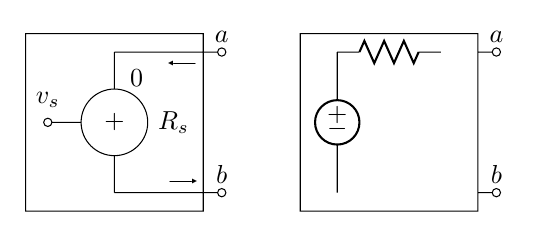
\includegraphics[scale=0.5]{images/fonteTensaoDominioW}
		\centering
		\caption*{Fonte: Modificado de \cite{Bogason2017}}
	\end{figure}
	
		%=========================================================================
		\subsubsection{Fonte de corrente com resistência não nula}
		%=========================================================================
	
	Assim como acontece para fontes de tensão, fontes de correntes independentes tem uma relação instantânea entre onda incidente e onda refletida. Por isso é interessante o uso de fontes de corrente em paralelo com resistores, conforme o circuito da Figura \ref{figFonteCorrenteModelada}. As relações entre as grandezas no domínio K para esse circuito são dadas na Equação \ref{TBD}:
	
	\begin{equation}
		\label{eqFonteCorrenteDominioK}
		V = (I + I_s).R_s
	\end{equation}
	
	\begin{figure}[h]
		\label{figFonteCorrenteModelada}
		\caption{Fonte de tensão com resistor em série a ser modelada}
		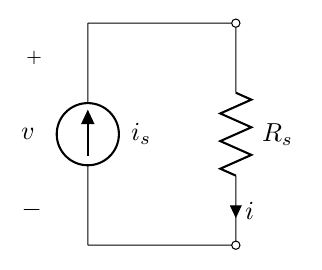
\includegraphics[scale=0.5]{images/fonteCorrenteModelada}
		\centering
		\caption*{Fonte: Modificado de \cite{Bogason2017}}
	\end{figure}
	
	Novamente se utilizando das relações nas Equações \ref{eqTensaoDefinicao} e \ref{eqCorrenteDefinicao} tem-se a relação entre onda incidente e onda refletida indicada na Equação \ref{eqFonteCorrenteDominioW} :
	
	\begin{equation}
		\label{eqFonteCorrenteDominioW}
		B = 2.I_s.\frac{R_p.R_s}{R_p+R_s}-a.\frac{R_p-R_s}{R_p+R_s}
	\end{equation}
	
	Novamente, para evitar uma relação instantânea entre onda incidente e onda refletida se define $R_p = R_s$ de maneira que essa fonte de corrente pode ser descrita no domínio W conforme as Equações \ref{eqBFonteCorrente} e \ref{eqRFonteCorrente} e na Figura \ref{figFonteCorrenteDominioW} é mostrado seu funcionamento e o símbolo que será usado para este componente no domínio W.
	
	\begin{equation}
		\label{eqBFonteCorrente}
		B = I_s.R_s
	\end{equation}
	
	\begin{equation}
		\label{eqRFonteCorrente}
		R_p = R_s
	\end{equation}
	
	\begin{figure}[h]
		\label{figFonteCorrenteDominioW}
		\caption{Funcionamento interno e símbolo de uma fonte de corrente com resistência em paralelo no domínio W}
		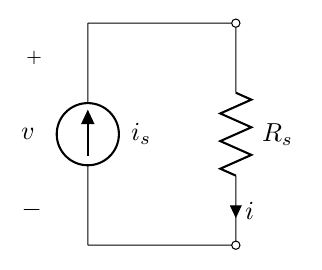
\includegraphics[scale=0.5]{images/fonteCorrenteModelada}
		\centering
		\caption*{Fonte: Modificado de \cite{Bogason2017}}
	\end{figure}
	
	
	\subsection{Conexões no domínio W}
	\label{secConexoesNoDominioW}
	
	\subsection{Amplificadores operacionais no domínio W}
	\subsection{Não linearidades no domínio W}
	
	\section{Espaço de Estados}

%=========================================================================
% METODOLOGIA EXPERIMENTAL
	\chapter{Metodologia Experimental}
	
	\section{Pedais a serem modelados}
	
	\section{Modelamento em filtro digital de onda}
	
	\section{Código spice do circuito}
%=========================================================================

%=========================================================================
% RESULTADOS E DISCUSSÕES
	\chapter{Resultados}
	
	\section{Resultados circuito 1}
	
	\section{Resultados circuito 2}
	
%=========================================================================

%=========================================================================
% CONCLUSÃO
	\chapter{Conclusões}
%=========================================================================

%=========================================================================
% PROPOSTA DE TRABALHOS FUTUROS
	\chapter{Propostas de Trabalhos Futuros}
%=========================================================================

%=========================================================================
% REFERÊNCIAS BIBLIOGRÁFICAS
	\postextual
	\bibliography{references}
%=========================================================================

%=========================================================================
% APÊNDICES
	\begin{apendicesenv}
	\partapendices
%=========================================================================
\end{apendicesenv}

%=========================================================================
% ANEXOS
	\begin{anexosenv}
	\partanexos
%=========================================================================
\end{anexosenv}

\end{document}
